\documentclass{beamer}

\usetheme{Madrid}
\usecolortheme{default}

\usepackage[spanish]{babel}

\setbeamertemplate{navigation symbols}{}
% siguiente punto transparente
\setbeamercovered{transparent}


% nombre de la sección arriba
\setbeamertemplate{headline}{
  \leavevmode%
  \hbox{%
    \begin{beamercolorbox}[wd=\paperwidth,ht=2.5ex,dp=1ex,center]{section in head/foot}%
      \insertsectionhead
    \end{beamercolorbox}%
  }%
}

% Código Lean
\usepackage{listings}

\usepackage{color}
\definecolor{keywordcolor}{rgb}{0.8, 0.1, 0.1}   % red
\definecolor{tacticcolor}{rgb}{0.0, 0.4, 0.9}    % blue
\definecolor{commentcolor}{rgb}{0.4, 0.4, 0.4}   % grey
\definecolor{symbolcolor}{rgb}{0.0, 0.4, 0.9}    % blue
\definecolor{sortcolor}{rgb}{0.1, 0.5, 0.1}      % green
\definecolor{attributecolor}{rgb}{0.7, 0.1, 0.1} % red
\definecolor{backgroundcolor}{rgb}{1, 1, 1} % light grey
\definecolor{contextcolor}{rgb}{0.9, 0.4, 0.1} %orange
\definecolor{bordercolor}{rgb}{0.5, 0.5, 0.5}
\definecolor{inlinecodecolor}{rgb}{0.92, 0.92, 0.92}

\def\lstlanguagefiles{../Memoria/lstlean.tex}

% Título
\title{Formalización de las matemáticas con Lean.}
\subtitle{Un caso de estudio: Resultados de Topología General.}
\author{Pepa Montero Jimena}
\institute[]{Facultad de Ciencias Matemáticas}
\date{Julio de 2025}


% ^ PREAMBLE

\begin{document}

% Código Lean
\lstset{language=lean, backgroundcolor=\color{backgroundcolor}}

% Frame con la sección

\AtBeginSection[]
{
  \begin{frame}{Índice}
    \tableofcontents[currentsection,hideothersubsections]
  \end{frame}
}


% Título
\frame{\titlepage}



\section{Introducción}

\begin{frame}{Motivación}
  \begin{itemize}
    \item Intersección entre matemáticas y computación
    \item Topología general
    \item Herramienta: Lean 4
  \end{itemize}
\end{frame}

\begin{frame}{Objetivos}
  \begin{itemize}
    \item Aprendizaje de Lean
    \item Formalización de un resultado relevante
    \begin{itemize}
      \item Lema de Urysohn
    \end{itemize}
    \item Ventajas y dificultades de la verificación formal
  \end{itemize}
\end{frame}

\begin{frame}{Plan de trabajo}
  \begin{itemize}
    \item Aprendizaje básico de Lean
    \begin{itemize}
      \item Lean at CompluMates 2023
      \item Formalising Mathematics by Kevin Buzzard
    \end{itemize}
    \item Resultados de topología general
    \item Formalización del Lema de Urysohn
    \begin{itemize}
      \item Comparación con la de Mathlib
    \end{itemize}
  \end{itemize}
\end{frame}

\section{Lean Theorem Prover}


\begin{frame}[fragile]{La base fundacional de Lean}

  \begin{center}
    \large{Cálculo de Construcciones Inductivas}
  \end{center}

  \begin{itemize}
    \item Teoría de tipos
  \end{itemize}

  \begin{lstlisting}
    #check 3    -- 3 : ℕ    
    #check ℕ    -- ℕ : Type
    #check ℝ → ℝ    -- ℝ → ℝ : Type \end{lstlisting}

  \begin{itemize}
    \item Cálculo lambda
  \end{itemize}

  \begin{lstlisting}
    def f := fun n ↦ n + 2
    #check f    -- ℕ → ℕ
    #eval f 3    -- 5 \end{lstlisting}

  \begin{itemize}
    \item Tipos dependientes
  \end{itemize}

  \begin{lstlisting}
    #check List    -- List.{u} (α : Type u) : Type u
    #check List ℝ    -- List ℝ : Type
    #check List.nil    -- {α : Type u} → List α
                       -- Π α : Type, List α \end{lstlisting}

\end{frame}


\begin{frame}[fragile]{La base fundacional de Lean}

  \begin{center}
    \large{Proposiciones y demostraciones}
  \end{center}

  \begin{itemize}
    \item Correspondencia de Curry-Howard
  \end{itemize}

  $$
  \begin{array}{rcl}
    \text{proposiciones} & \longleftrightarrow & \text{tipos} \\
    \text{demostraciones} & \longleftrightarrow & \text{programas}
  \end{array}
  $$

  \begin{lstlisting}
    #check Prop    -- Prop : Type
    variable (P : Prop)
    #check P    -- P : Prop
    variable (D : P)
    #check D    -- D : P \end{lstlisting}

\end{frame}

\begin{frame}[fragile]{Uso práctico de Lean}
  \begin{itemize}
    \item Modo táctico
    \item Lean InfoView
  \end{itemize}

  \hspace{1cm}

  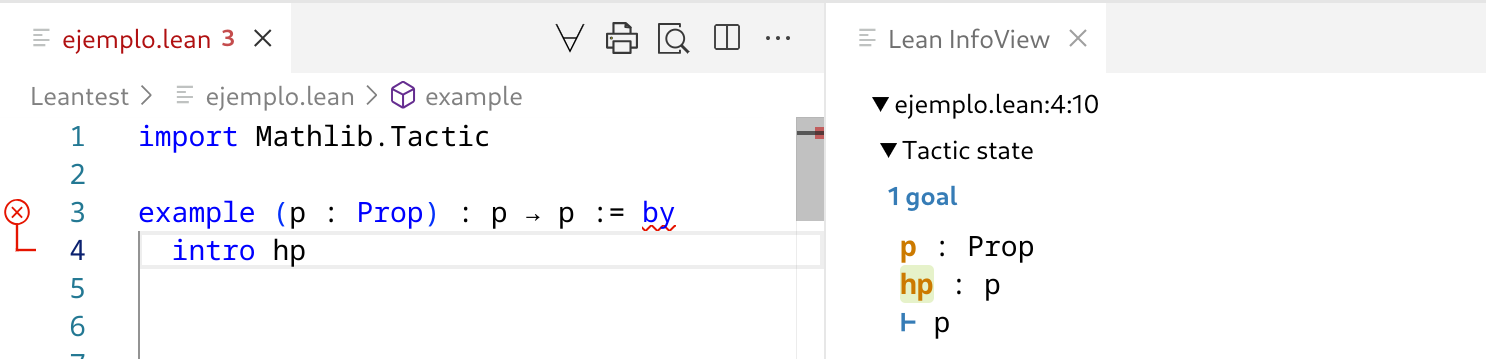
\includegraphics[width=\linewidth]{figuras/infoview.png}

  \hspace{1cm}

  \begin{itemize}
    \item Utilizar términos
  \end{itemize}

  \begin{lstlisting}
    example (p : Prop) : p → p := fun hp ↦ hp \end{lstlisting}
\end{frame}

\section{Espacios Topológicos en Lean}

\begin{frame}[fragile]{Espacios topológicos}
  \begin{block}{Definición (Espacio topológico)}
    Sea $X$ un conjunto y $\mathcal{T}$ una colección de subconjuntos de $X$ de forma que
    \begin{enumerate}
      \item Los conjuntos $\emptyset$ y $X$ pertenecen a $\mathcal{T}$.
      \item Cualquier intersección finita de elementos de $\mathcal{T}$ pertenece a $\mathcal{T}$.
      \item Cualquier unión arbitraria de elementos de $\mathcal{T}$ pertenece a $\mathcal{T}$.
    \end{enumerate}
    Entonces diremos que $(X, \mathcal{T})$ es un \textnormal{espacio topológico}.
  \end{block}

  \begin{lstlisting}
  class TopologicalSpace (X : Type u) where
    IsOpen : Set X → Prop
    isOpen_univ : IsOpen Set.univ
    isOpen_inter : ∀ s t, IsOpen s → IsOpen t → IsOpen (s ∩ t)
    isOpen_sUnion : ∀ s, (∀ t ∈ s, IsOpen t) → IsOpen (⋃₀ s) \end{lstlisting}
\end{frame}

\begin{frame}[fragile]{Espacios normales}
  
  \begin{block}{Definición (Espacio normal)}
     Sea $X$ un espacio topológico. Diremos que $X$ es un espacio \textnormal{normal} si para cada par de cerrados disjuntos $C, D \subseteq X$ existen abiertos disjuntos $U$ y $V$ en $X$ tales que separan $C$ y $D$, es decir, $C \subseteq U$ y $D \subseteq V$.
  \end{block}

  \begin{lstlisting}
  def NormalSpace {X : Type} (T : TopologicalSpace X) : Prop :=
    ∀ C : Set X, ∀ D : Set X,
    IsClosed C → IsClosed D → Disjoint C D →
    ∃ U : Set X, ∃ V : Set X,
      IsOpen U ∧ IsOpen V ∧ C ⊆ U ∧ D ⊆ V ∧ Disjoint U V \end{lstlisting}
\end{frame}

\begin{frame}[fragile]{Caracterización de espacios normales}
  
  \begin{block}{Proposición}
    Sea $X$ un espacio topológico. $X$ es normal si y sólo si para cada abierto $U$ y cada cerrado $C$ de $X$ tales que $C \subseteq U$, existe un abierto $V \subset X$ de forma que $C \subseteq V \subseteq \overline{V} \subseteq U$.
  \end{block}

  \begin{lstlisting}
  lemma characterization_of_normal {X : Type}
      (T : TopologicalSpace X) :
    NormalTopoSpace T ↔
      ∀ U : Set X, ∀ C : Set X,
        IsOpen U → IsClosed C → C ⊆ U →
      ∃ V : Set X,
        IsOpen V ∧ C ⊆ V ∧ (Closure V) ⊆ U := by sorry \end{lstlisting}

\end{frame}

\section{El Lema de Urysohn}

\begin{frame}[fragile]{El Lema de Urysohn}

  \begin{block}{Lema de Urysohn}
    Sea $(X, \mathcal{T})$ un espacio topológico. $X$ es un espacio normal si y solo si para cada par de conjuntos cerrados disjuntos $C_1$ y $C_2$ en $X$, existe una función $f : X \to [0, 1]$ de manera que $f(C_1) = \{0\}$ y $f(C_2) = \{1\}$.
  \end{block}

  \begin{lstlisting}
  lemma Urysohn {X : Type} (T : TopologicalSpace X)
      {Y : Set ℝ} {hY : Y = Set.Icc 0 1}
      [T' : TopologicalSpace ℝ] (hT' : T' = UsualTopology)
      {R : TopologicalSpace Y} {hR : R = TopoSubspace T' Y} :
    NormalSpace X ↔
      ∀ C1 : Set X, ∀ C2 : Set X, C1 ≠ ∅ → C2 ≠ ∅ →
      IsClosed C1 → IsClosed C2 → Disjoint C1 C2 →
      ∃ f : X → Y,
        Continuous f ∧
        f '' C1 = ({⟨0, by simp [hY]⟩} : Set Y) ∧
        f '' C2 = ({⟨1, by simp [hY]⟩} : Set Y) := by sorry \end{lstlisting}
  
\end{frame}

\begin{frame}{Idea de la demostración}

  Sea $X$ un espacio normal, $C_1$ y $C_2$ cerrados disjuntos.
  
  \begin{block}{Recordatorio: caracterización de espacios normales}
    $$
    \left.
    \begin{array}{l}
    U \text{ abierto} \\
    C \text{ cerrado} \\
    C \subseteq U
    \end{array}
    \right\}
    \quad \implies \quad
    \exists V \text{ abierto}, \quad C \subseteq V \subseteq \overline{V} \subseteq U
    $$
  \end{block}

  Sucesión de abiertos $\{U_k : k \in \mathbb{Q} \cap [0, 1]\}$:

  \begin{itemize}
    \item $U_1 = C_2^c$
    \item $U_0$ es tal que $C_1 \subseteq U_0 \subseteq \overline{U_0} \subseteq U_1$
    \item $U_{\frac{1}{2}}$ es tal que $\overline{U_0} \subseteq U_{\frac{1}{2}} \subseteq \overline{U_{\frac{1}{2}}} \subseteq U_1$
  \end{itemize}

  tal que
  \begin{equation}
  p < q \implies \overline{U_p} \subseteq U_q \tag{$\star$} \label{eq:star}
  \end{equation}

  Tomamos la función $f : X \to [0, 1]$
  $$
  f(x) = \inf \{p \in \mathbb{Q} : x \in U_p\}
  $$

\end{frame}

\begin{frame}{Principales dificultades de la formalización}
  
  \begin{itemize}
    \item Construcción de la sucesión de abiertos
    \item Demostración de que la sucesión es creciente (\ref{eq:star})
  \end{itemize}

  \hspace{1cm}

  Según nuestra idea:

  $$
    \left.
    \begin{array}{l}
    U_p, U_q \text{ definidos} \\
    p < r < q
    \end{array}
    \right\}
    ~ \longrightarrow ~
    \text{quiero } U_r \text{ con } \overline{U_p} \subseteq U_r \subseteq \overline{U_r} \subseteq U_q
  $$

  pero ¿$\overline{U_p} \subseteq U_q$?

  \hspace{1cm}

  
  \uncover<2>{
  Soluciones:

  \begin{itemize}
    \item Construir la sucesión parcialmente
    \item Numerar los racionales
    \item Utilizar inducción bien fundada sobre el orden lexicográfico de $\mathbb{N} \times \mathbb{N}$
  \end{itemize}
  }

\end{frame}

\section{Conclusiones}

\begin{frame}{Conclusiones}
  
  \begin{itemize}
    \item Simplificación y revisión constante
    \item Reutilización de resultados de Mathlib
    \item Uso de herramientas de búsqueda
    \item Comprensión de la materia
    \item Conversión del papel a Lean
    \begin{itemize}
      \item Urysohn en Mathlib
    \end{itemize}
  \end{itemize}

\end{frame}

\begin{frame}{Posibles mejoras y ampliaciones}
  
  \begin{itemize}
    \item Uso sitemático de definciones de Mathlib
    \item Documentación del código
    \item Topology Game
    \item Verificación de programas
    \begin{itemize}
      \item Máster en Métodos Formales en Ingeniería Informática
    \end{itemize}
  \end{itemize}

\end{frame}


\begin{frame}
  \centering
  \Huge
  \textbf{¡Gracias!}

  \vspace{1cm}

  \Large \insertshorttitle

  \Large \insertshortsubtitle

  \vspace{0.5cm}

  \large \insertauthor


\end{frame}

\end{document}

